\documentclass[11pt]{article}

\oddsidemargin0cm
\topmargin-2cm     %I recommend adding these three lines to increase the 
\textwidth16.5cm   %amount of usable space on the page (and save trees)
\textheight23.5cm  

\newcommand{\question}[2] {\vspace{.25in} \fbox{#1} #2 \vspace{.10in}}
\renewcommand{\part}[1] {\vspace{.10in} {\bf (#1)}}

\usepackage{graphicx}
\usepackage{amssymb,amsmath}

\begin{document}

\medskip                        % Skip a "medium" amount of space
                                % (latex determines what medium is)
                                % Also try: \bigskip, \littleskip


\begin{center}                  % Center the following lines
  {\Large Introduction to the Theory of Computation \\ Homework \#3} \\
  Brian Gianforcaro \\
  \date \\
\end{center}

\ttfamily

\question{1}{}

\part{a}
   $0^{*}1^{*}$  

\part{d}
   $(0 \cup 1) \cup (0 \cup 1) \cup (0 \cup 1)0$  

\part{i}
   $(10)^{*}\cup(11)^{*}$  


\part{l}
   $(0^{2})^{*}\cup{0}^{*}(11){0}^{*}$  


\part{m}
 $\emptyset$


\part{n}
   $((0^{*}{1}^{*})^{*}(1^{*}{0}^{*})^{*})^{+} $ 


\question{2}{}

   ${\epsilon} {\cup} 001(0-1)^{*}{\cup}(0-1)^{*}11$  

\question{3}{}

   $({b}^{*} \cup aaa \cup aa \cup a ){b}^{*}aaaa{b}^{*}({b}^{*} \cup aaa \cup aa \cup a )$  

\question{4}{}

 \part{a}
  \begin{figure}[h!]
    \begin{center}
      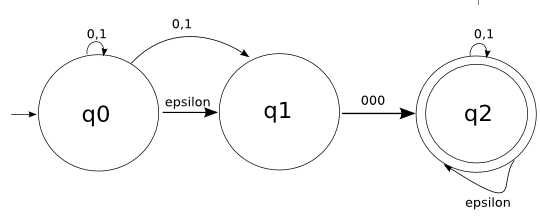
\includegraphics[scale=0.40]{19a.png}
    \end{center}
  \end{figure}


\pagebreak 
 \part{b}
  \begin{figure}[h!]
    \begin{center}
      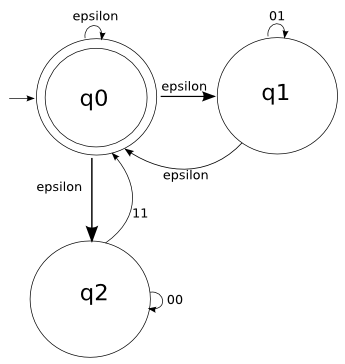
\includegraphics[scale=0.40]{19b.png}
    \end{center}
  \end{figure}

 \part{c}
  \begin{figure}[h!]
    \begin{center}
      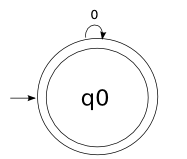
\includegraphics[scale=0.40]{19c.png}
    \end{center}
  \end{figure}


\question{5}{Proof: By Structural Induction}
\begin{center}
  \begin{itemize}
    \item Observe $x \epsilon {\Sigma}^{*}, L = L(R)$
    \item Assume R is over $\Sigma$

    $ x \epsilon {\Sigma}^{*} $ 

    $ L(R) = {x} $ 


  \end{itemize}
\end{center}

\indent $\Box$

\question{6}{Proof: By Mathematical Induction}
\begin{center}
  \begin{itemize}

    \item Observe $n \epsilon \mathcal{N}, L \subset {\Sigma}^{*}$

    \item Suppose $|L| = n $

    $ L(R) = {x} $

    $ |L(R)| = 1 $

    $ |L(R)| = |L| $

    There fore R exists such that L(R) = L

  \end{itemize}
\end{center}

\indent $\Box$

\end{document}
